%%%%%%%%%%%%%%%%%%%%%%%%%%%%%%%%%%%%%%%%%%%%%%%%%%%%%%%%%%%%%%%%%%%
%%% Documento LaTeX 																						%%%
%%%%%%%%%%%%%%%%%%%%%%%%%%%%%%%%%%%%%%%%%%%%%%%%%%%%%%%%%%%%%%%%%%%
% Título:		Capítulo 3
% Autor:  	Ignacio Moreno Doblas
% Fecha:  	2014-02-01, actualizado 2019-11-11
% Versión:	0.5.0
%%%%%%%%%%%%%%%%%%%%%%%%%%%%%%%%%%%%%%%%%%%%%%%%%%%%%%%%%%%%%%%%%%%
% !TEX root = A0.MiTFG.tex

\section{Primera iteración: El núcleo}
    \subsection{Resumen}

        Esta primera iteración está centrada en la codificación de la estructura básica de la aplicación, creando durante ella la infraestructura que servirá de apoyo para todas las funcionalidades que se implementen en las sucesivas iteraciones, llamado comúnmente como ``Core application''. 

        Para dar esta iteración por finalizada, la aplicación del panel deberá ser capaz de enviar las muestras de ECG hacia la plataforma de muestreo y está a su vez ser capaz de recibirlas y enviarlas de vuelta al panel, verificando así la comunicación en el doble sentido.

    \subsection{Requisitos}

        Los requisitos a realizar en esta iteración son el 1.1, el 2.2 y el 2.1 de la tabla de requisitos iniciales. (Tabla \ref{tab:Requisitos}) Estos requisitos dan lugar al siguiente desglose de tareas y subtareas:

        \begin{enumerate}
                \item Introducir señales de pruebas.
                \begin{enumerate}
                        \item Lectura de un fichero de datos con muestras de ECG.
                        \item Envío de las lecturas a la plataforma de testeo a la frecuencia original de muestreo.
                        \item Interfaz de usuario básica para gestionar la lectura del fichero.
                \end{enumerate}
                \item Entrada de datos en tiempo real.
                \begin{enumerate}
                        \item Buscar la manera de realizar el análisis de manera continuada sin dejar de recibir nuevos datos en el proceso.
                \end{enumerate}
                \item Protocolo de comunicación.
                \begin{enumerate}
                        \item Definir el protocolo de comunicación a emplear.
                \end{enumerate}
        \end{enumerate}

    \subsection{Desarrollo}

        El primer paso fue la investigación de las bases de datos fisiológicos, concretamente bases de datos con muestras de ECG estandarizadas y ampliamente extendidas. Destacando la MIT-BIH Arrythmia Database (TODO: citar https://www.physionet.org/content/mitdb/1.0.0/). Accediendo a los datos a través del repositorio de Physionet, haciendo uso de su propia API para descargar los datos directamente desde matlab. (TODO: Citas) De este modo, con un simple script, es posible convertir cualquier muestra de datos procedente de dicho repositorio en un fichero de texto estandarizado para la entrada de datos del entorno de pruebas.

        \begin{figure} 
                \centering
                        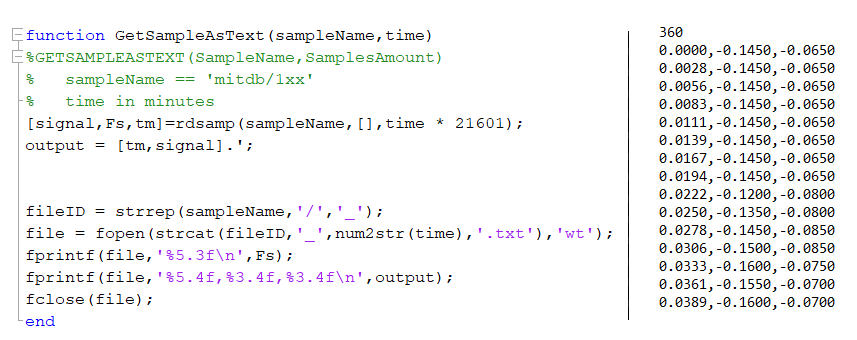
\includegraphics[width =\linewidth]{figuras/MatlabFunc.png}
                \caption{Función de Matlab para extraer los datos del repositorio y formatearlos como texto}
                \label{fig:MAtlabFunc}
        \end{figure}

        El siguiente paso consiste en leer dichos ficheros de texto desde el panel de usuario y preparar los datos para enviarlos al dispositivo de pruebas. Este proceso tiene dos puntos claves, la lectura debe ser periódica y su frecuencia debe ser igual que la frecuencia de muestreo de las muestras. Para lograr este cometido se ha desarrollado un script siguiendo la estructura del diagrama \ref{fig:SimpleFileRead}. 

        \begin{figure}[H]  
                \centering
                        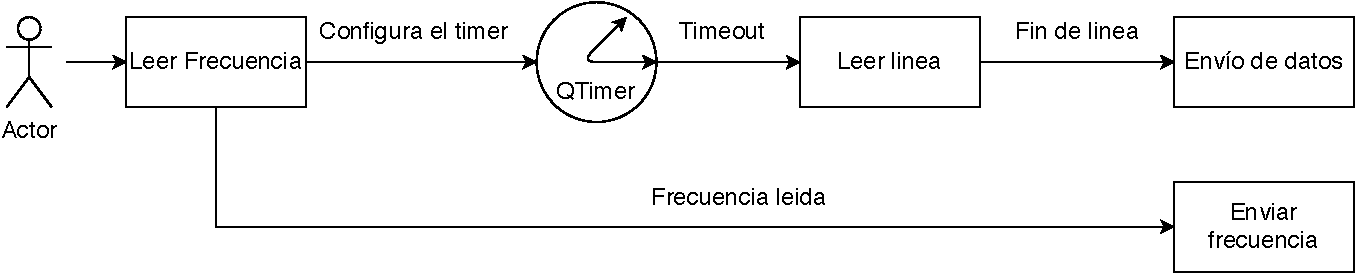
\includegraphics[width =\linewidth]{figuras/SimpleFileRead.pdf}
                \caption{Diagrama de lectura de ficheros simplificado}
                \label{fig:SimpleFileRead}
        \end{figure}

        Para sincronizar las partes del script y garantizar la compatibilidad y sincronismo con futuras funcionalidades del panel de control se hace uso de los SLOT y las SIGNAL de Qt. Estos elementos son el pilar fundamental de las aplicaciones desarrolladas con Qt ya que actúan como canales de mensajes, permitiendo la sincronización de todas las funciones de la aplicación sin caer en fuertes restricciones por acoplamiento de las diferentes funcionalidades.

        Como se puede ver en el diagrama \ref{fig:CompleteFileRead} se han añadido también diferentes entradas para que el usuario interaccione. Estas son una rueda selectora para configurar la frecuencia de forma manual, un botón para realizar la lectura de la frecuencia de muestreo directamente desde el fichero y un tercero que daría comienzo a la prueba. En la figura \ref{fig:frecKnob} se puede ver la disposición de estos elementos.

        \begin{figure} [H] 
                \centering
                        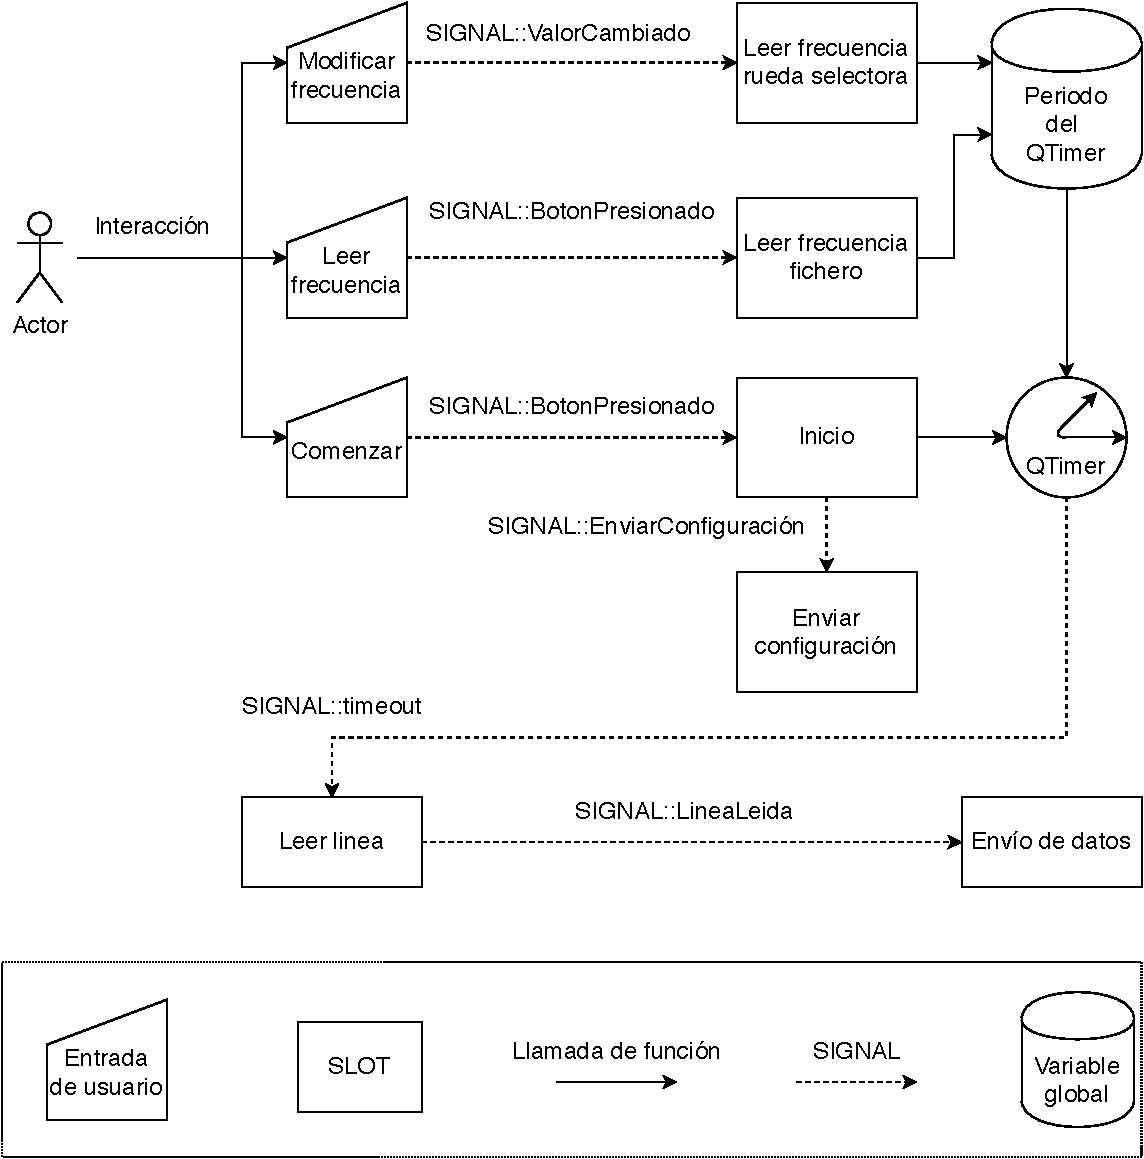
\includegraphics[width =\linewidth]{figuras/CompleteFileRead.pdf}
                \caption{Diagrama de lectura de ficheros en QT}
                \label{fig:CompleteFileRead}
        \end{figure}

        Antes de continuar con la información sobre el envío de los datos, es necesario detenerse en la gestión del tiempo real y el sincronismo dentro del dispositivo de pruebas, concretamente la Tiva (TM4C123GXL). Para esta finalidad se ha hecho uso de un sistema operativo de tiempo real de software libre llamado FREERTOS (TODO: Cita). Gracias a él se pueden gestionar y sincronizar tareas asignándoles diferentes prioridades, solucionando el problema de tener que gestionar las comunicaciones a la vez que se realizan las pruebas de rendimiento, ganando en el proceso además mayor independencia entre las tareas reduciendo acoplamientos.
        
        \begin{figure}[H]
                \centering
                        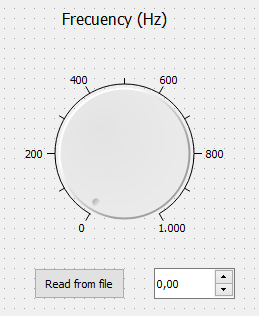
\includegraphics[width =0.4\linewidth]{figuras/FrecKnob.png}
                \caption{Selector de frecuencias y lectura del fichero}
                \label{fig:frecKnob}
        \end{figure}

        Para la comunicación entre el dispositivo de pruebas y el panel de usuario se hace uso de un puerto serie. Para garantizar la correcta transmisión de los datos se emplean dos mecanismos muy extendidos, checksum y byte stuffing. Pudiendo representar el protocolo en el diagrama \ref{fig:frame}. Cada salto de línea representa cada nueva etapa del protocolo de envío. El ejemplo expuesto contiene un byte de datos que coincide con el byte de final de trama, representado como “END”, a fin de ejemplificar el funcionamiento del método de stuffing escogido.

        \begin{figure}[H]
                \centering
                        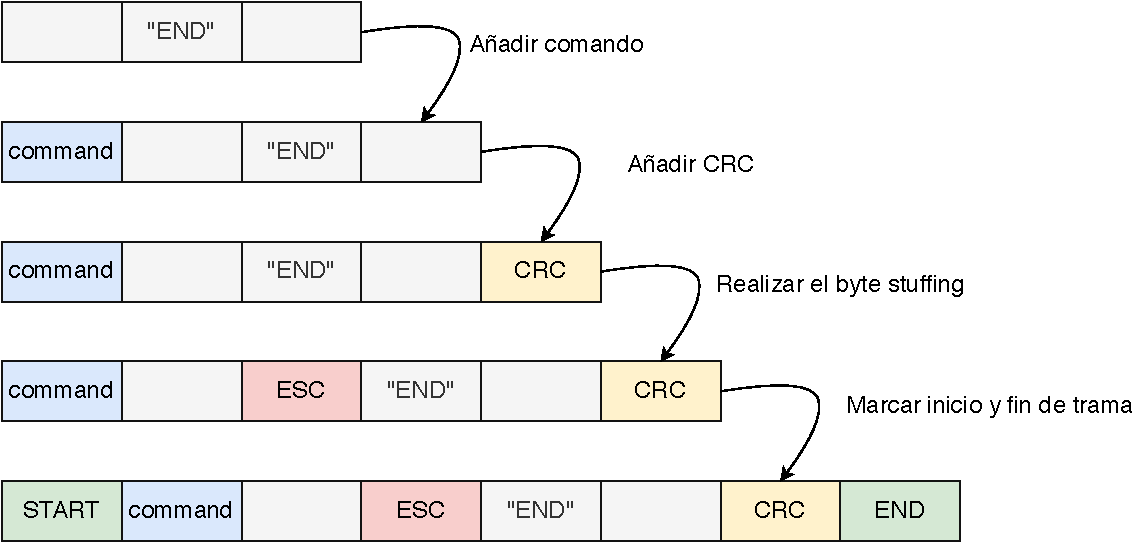
\includegraphics[width = \linewidth]{figuras/ProtocoloCom.pdf}
                \caption{Proceso construcción de trama}
                \label{fig:frame}
        \end{figure}

    \subsection{Pruebas}

        Para testear la lectura de ficheros en Qt se han implementado una serie de tests unitarios con el objetivo de verificar las lecturas, pero además, de verificar que ante entradas de datos erróneas como ficheros mal formateados el sistema reacciona de forma correcta.

        Los casos sometidos a test han sido:

        \begin{itemize}
                \item Lectura correcta de la frecuencia desde el fichero
                \item Lectura incorrecta de la frecuencia desde el fichero
                \item Lectura correcta de una línea de datos
                \item Lectura incorrecta de una línea de datos
        \end{itemize}

        Para el protocolo el proceso ha sido similar, si es capaces de codificar y decodificar un mensaje, donde entre en juego la necesidad de emplear el bit Stuffing, entonces debe ser capaz de codificar y decodificar cualquier mensaje.

        Para comprobar la transmisión de los datos entre el panel y el dispositivo de prueba se ha optado por un test de carácter más empírico. Si se puede enviar en tiempo real y recibir de vuelta la señal deseada sin que los datos se distorsionen, se puede concluir que el sistema de transmisión funciona correctamente.

        (TODO: Imagen de los dos ECG)


    \subsection{Conclusiones}

        Tras la realización de esta iteración quedan sentadas las bases para el correcto desarrollo del proyecto. A su vez se hizo presente la necesidad de implementar una nueva funcionalidad.

        La inclusión de un mecanismo para que el usuario pueda seleccionar de manera fácil e intuitiva la muestra de señal que desea emplear para las pruebas. Esta funcionalidad ha sido incluida en la tabla de requisitos finales con el código 1.5. de la sección de conclusiones finales. (TODO: Referencia a la tabla final)

        De la realización de los test también se observó la necesidad de incluir algún tipo de mecanismo de mensajes para notificar a los usuarios los errores o advertencias que se produzcan en el panel de control. Esta funcionalidad se ha incluido en la tabla de requisitos finales con el código 1.6. de la sección de conclusiones finales (TODO: Referencia a la tabla)
        